\chapter{Results and Analysis}
\label{ch:ResultsAnalysis}
In this chapter, the performance of the trained models is analyzed and discussed. The main focus is on the final MLP regressor model, which was found to be the best performing model across multiple criteria. The selection of the MLP regressor is supported by the results shown in \autoref{fig:ModelSRCC}, which presents a parallel coordinate plot comparing the best-performing models across all seven criteria and the overall SRCC.\par
\begin{figure}[ht]
    \centering
    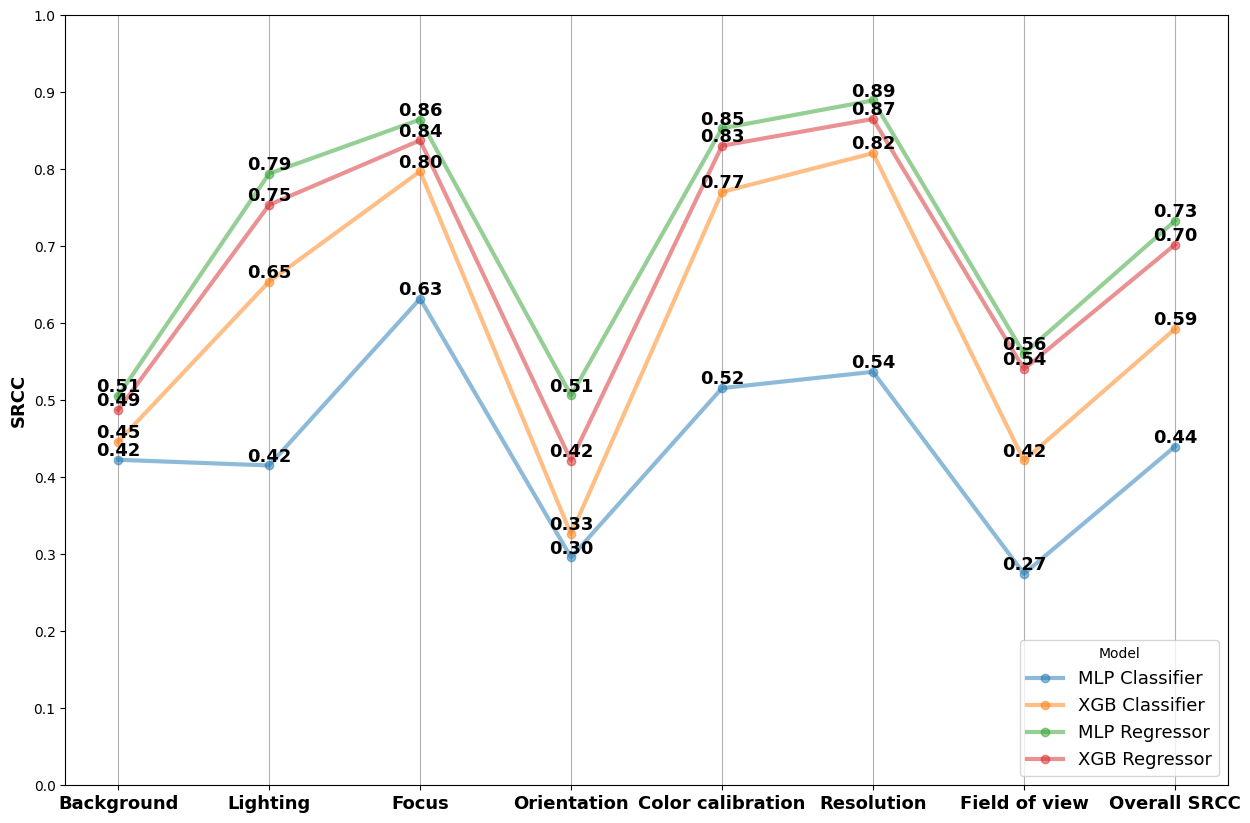
\includegraphics[keepaspectratio,width=15cm]{img/Model_SRCC.png}
    \caption{Parallel coordinate plot showing the best SRCC values for the four different models across the seven criteria and the overall SRCC. This plot highlights the performance of the MLP Regressor.}
    \label{fig:ModelSRCC}
\end{figure}
\noindent
The parallel coordinate plot shows that the MLP regressor consistently performs better than the other models across all criteria. Although all models perform similarly for different criteria, no model stands out in a specific criterion. This could be because the same features were used for every criterion, with only the target labels differing. \par
\vspace{\baselineskip}
\noindent
In addition to the parallel coordinate plot, \autoref{table:srcc_results} summarizes the cross-dataset evaluation results, showing the generalizability of the models. The table lists the models in the left column and their evaluation results on the SCIN and Fitzpatrick (F17K) datasets in the right columns. This table shows how well the models, trained on one dataset, perform when evaluated on another, providing insights into their robustness and adaptability. All data were synthetically distorted through the pipeline to ensure consistent evaluation conditions. \par
\begin{table}[h]
    \centering
    \begin{tabular}{|l|c|c|}
        \hline
        \textbf{Model} & \textbf{SCIN} & \textbf{F17K} \\
        \hline
        Combined MLP Regressor & \underline{0.66} & \underline{0.75} \\
        Combined XGB Regressor & 0.65 & 0.73 \\
        Combined XGB Classifier & 0.58 & 0.61 \\
        Combined MLP Classifier & 0.43 & 0.46 \\
        \hline
        F17K MLP Regressor & 0.54 & 0.69 \\
        SCIN MLP Regressor & 0.62 & 0.49 \\
        F17K XGB Regressor & 0.53 & 0.67 \\
        SCIN XGB Regressor & 0.61 & 0.48 \\
        SCIN MLP Classifier & 0.53 & 0.45 \\
        F17K MLP Classifier & 0.47 & 0.58 \\
        SCIN XGB Classifier & 0.54 & 0.43 \\
        F17K XGB Classifier & 0.46 & 0.59 \\
        \hline
    \end{tabular}
    \caption{Spearman’s Rank Correlation Coefficient (SRCC) of Different Models on SCIN and F17K Datasets. F17K refers to the Fitzpatrick17k dataset.}
    \label{table:srcc_results}
\end{table}
\noindent
Given these findings, the MLP regressor was chosen as the final model for further testing. The following sections will detail the performance of the MLP regressor on the test images, providing a clear analysis of its strengths and weaknesses in assessing image quality in teledermatology. \par

\section{Model Performance}
\label{sec:ModelPerformance}
To fully understand the model’s performance, both overall metrics and individual criteria performance were analyzed\footnote{from utils.visualization import print\_metrics}. \autoref{table:performance_metrics} shows the results for the final MLP regressor model evaluated on the 475 good quality Fitzpatrick images, which were synthetically distorted using the distortion pipeline. The results indicate that the model performs very well on focus, color calibration, and resolution, with low MAE, high R\textsuperscript{2}, SRCC, and Cohen’s Kappa values. However, the most problematic criteria are background and orientation. These metrics provide a comprehensive view of the model’s strengths and weaknesses, highlighting areas that may need improvement. \par
\begin{table}[h]
    \centering
    \begin{tabular}{|l|c|c|c|c|}
        \hline
        \textbf{Criteria} & \textbf{MAE} & \textbf{R\textsuperscript{2}} & \textbf{SRCC} & \textbf{Cohen's Kappa} \\
        \hline
        Background & 0.9684 & 0.2595 & 0.5422 & 0.4399 \\
        Lighting & 0.5726 & 0.6440 & 0.8028 & 0.7913 \\
        Focus & 0.4042 & 0.7385 & 0.8622 & 0.8568 \\
        Orientation & 0.9895 & 0.1824 & 0.4735 & 0.4102 \\
        Color calibration & 0.4905 & 0.7334 & 0.8622 & 0.8583 \\
        Resolution & 0.3642 & 0.7656 & 0.8722 & 0.8726 \\
        Field of view & 0.5474 & 0.5976 & 0.7710 & 0.7660 \\
        \hline
        \textbf{Overall} & \textbf{0.6195} & \textbf{0.5646} & \textbf{0.7507} & \textbf{0.7396} \\
        \hline
    \end{tabular}
    \caption{Performance Metrics for Each Distortion Criteria}
    \label{table:performance_metrics}
\end{table}

\vspace{\baselineskip}
\noindent
In addition to numerical metrics, visual tools were used to gain a clearer understanding of the model’s performance. For each criterion, a confusion matrix\footnote{from utils.visualization import plot\_all\_confusion\_matrices} was created. As shown in \autoref{fig:confusion_matrices} these matrices display where the model makes correct predictions and where it makes mistakes, showing a detailed view of its accuracy for each type of distortion. The confusion matrix also shows the comparison between the actual scores and the predicted scores. \par
\begin{figure}[ht]
    \centering
    \begin{subfigure}[b]{0.32\textwidth}
        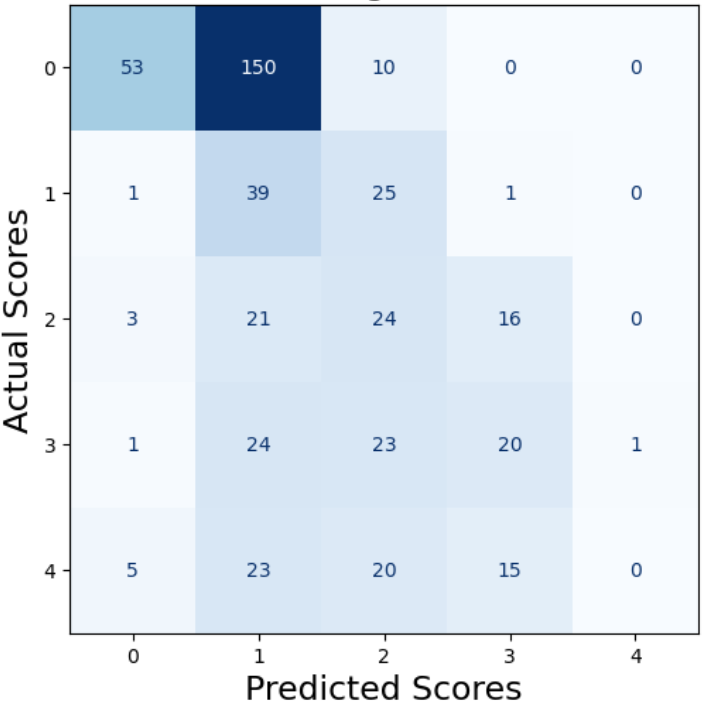
\includegraphics[width=\textwidth]{img/cm/bg.png}
        \caption{Background}
        \label{fig:cm_bg}
    \end{subfigure}
    \hfill
    \begin{subfigure}[b]{0.32\textwidth}
        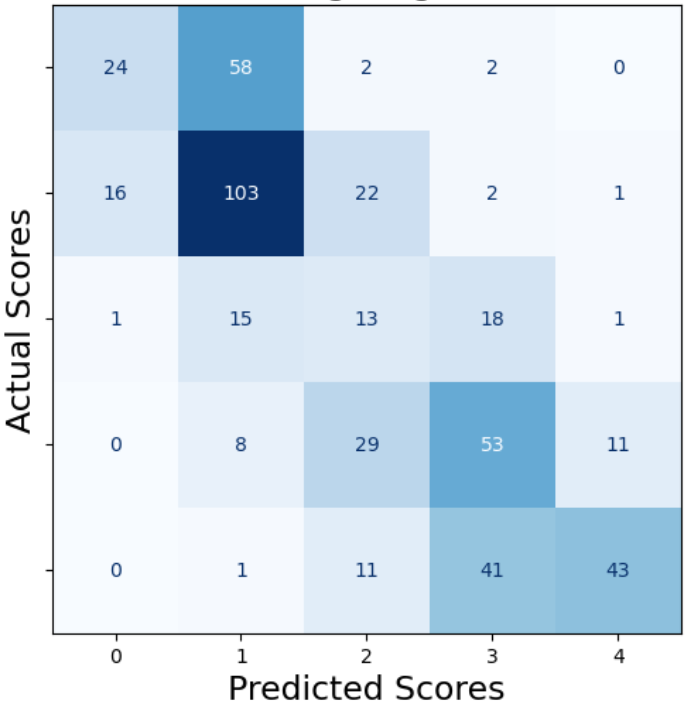
\includegraphics[width=\textwidth]{img/cm/light.png}
        \caption{Lighting}
        \label{fig:cm_light}
    \end{subfigure}
    \hfill
    \begin{subfigure}[b]{0.32\textwidth}
        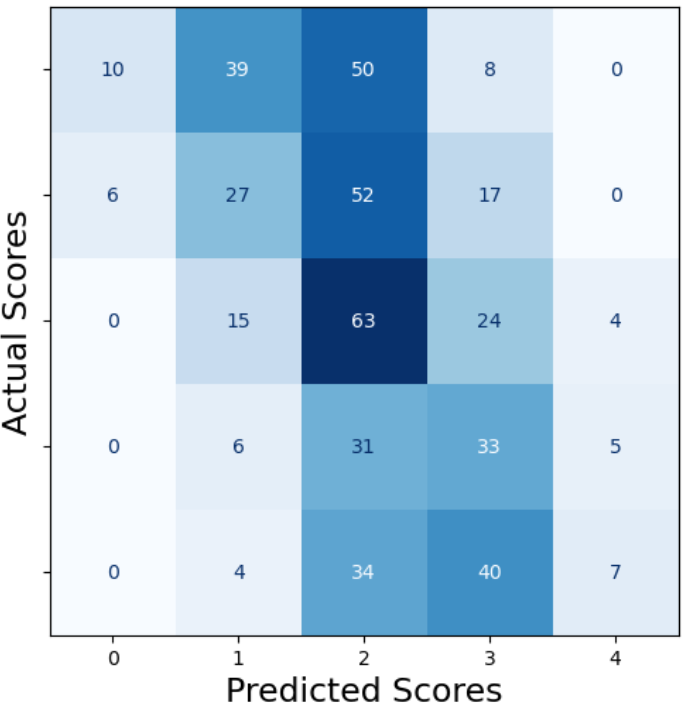
\includegraphics[width=\textwidth]{img/cm/orient.png}
        \caption{Orientation}
        \label{fig:cm_orient}
    \end{subfigure} 

    \begin{subfigure}[b]{0.24\textwidth}
        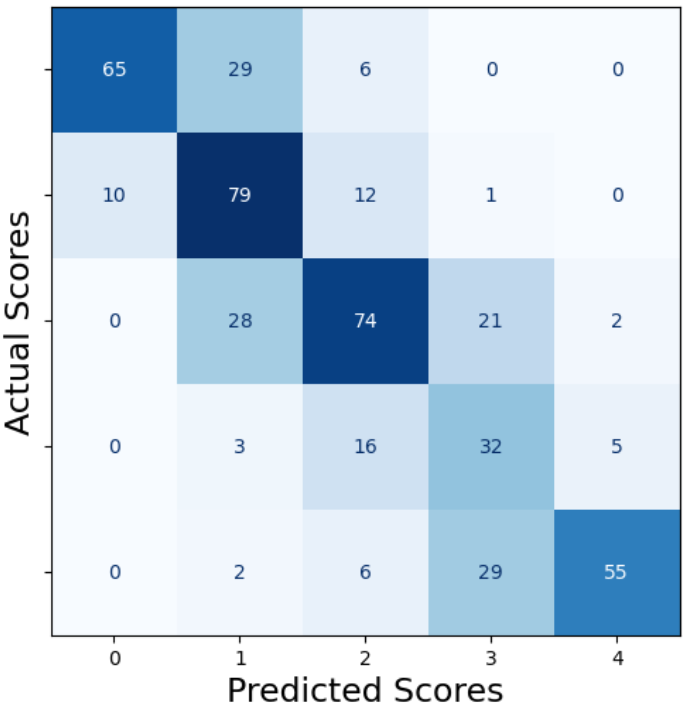
\includegraphics[width=\textwidth]{img/cm/foc.png}
        \caption{Focus}
        \label{fig:cm_foc}
    \end{subfigure}
    \hfill
    \begin{subfigure}[b]{0.24\textwidth}
        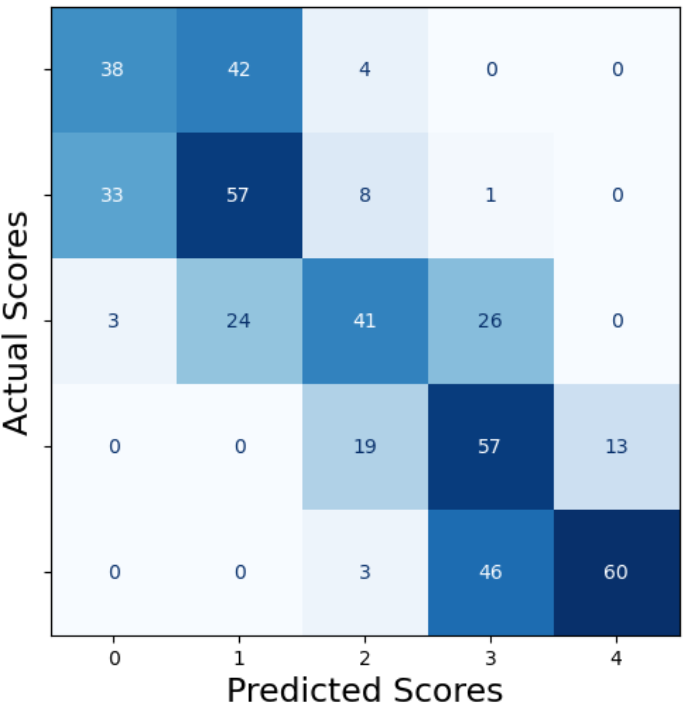
\includegraphics[width=\textwidth]{img/cm/cc.png}
        \caption{Color Calibration}
        \label{fig:cm_cc}
    \end{subfigure}
    \hfill
    \begin{subfigure}[b]{0.24\textwidth}
        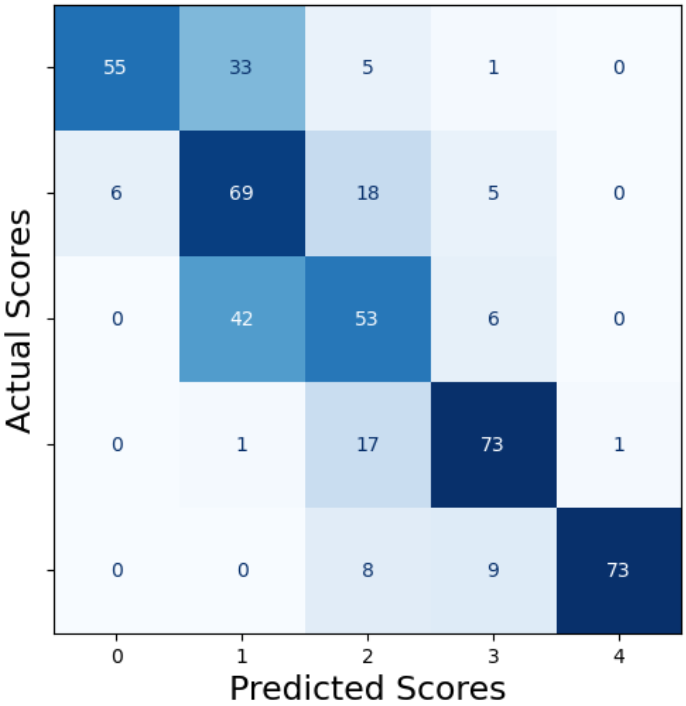
\includegraphics[width=\textwidth]{img/cm/res.png}
        \caption{Resolution}
        \label{fig:cm_res}
    \end{subfigure}
    \hfill
    \begin{subfigure}[b]{0.24\textwidth}
        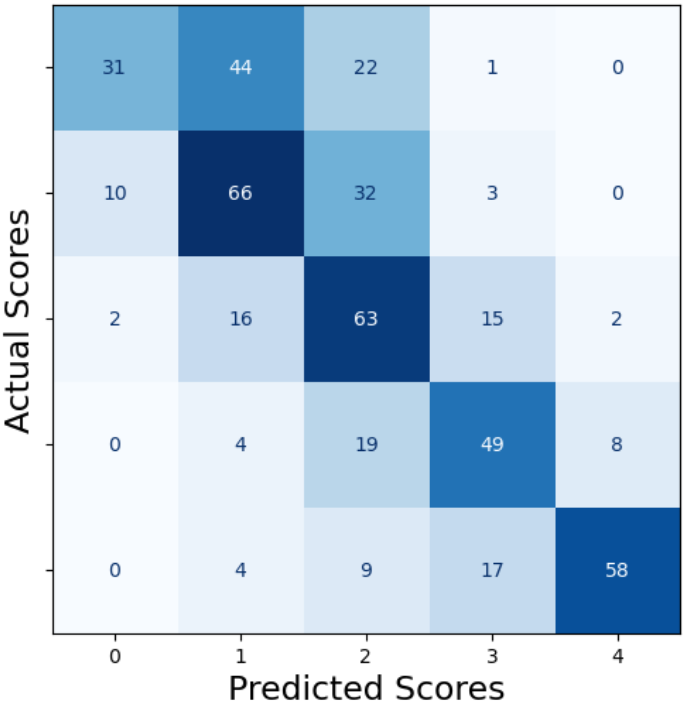
\includegraphics[width=\textwidth]{img/cm/fov.png}
        \caption{Field of View}
        \label{fig:cm_fov}
    \end{subfigure}
    \caption{Confusion matrices for the MLP Regressor model evaluated on the 475 images from the Fitzpatrick dataset. Each matrix corresponds to a specific distortion criterion and shows the actual scores on the y-axis and the predicted scores on the x-axis. Darker shades indicate higher counts, highlighting where the model's predictions match the actual values and where discrepancies occur.}
    \label{fig:confusion_matrices}
\end{figure}
\vspace{\baselineskip}
\noindent
Examining the confusion plots shows that the bottom row (Figure~\ref{fig:cm_foc} to~\ref{fig:cm_fov}) shows good performance, where the diagonal indicate correct predictions with only minor fluctuations. In contrast, the top row (Figure~\ref{fig:cm_bg} to~\ref{fig:cm_orient}) has more noticeable issues. For instance, \autoref{fig:cm_bg} shows that there are rarely predictions on the higher severity for background distortion. This is because, in the distortion pipeline, if the background proportion is less than 10\%, no color blocks are added, resulting in a 0 value for background distortion. This indicates many images were given a 0 for background distortion. Improving the training dataset to include more images with background could address this issue. \par
\vspace{\baselineskip}
\noindent
Orientation predictions, as shown in \autoref{fig:cm_orient}, is generally unsure and tend to cluster in the middle. This might be due to the various perspective changes (top, bottom, right, left) applied, making the model predict around the middle as it detects perspective distortions but not precisely which way and how strong. \par
\vspace{\baselineskip}
\noindent
Lighting predictions, as shown in \autoref{fig:cm_light}, are reasonably accurate, but errors may occur because the criteria include two opposite types of distortion: brightening and darkening the image. This could lead to mispredictions as the inherent distortions look opposite but have the same values for the criteria. \par
\vspace{\baselineskip}
\noindent
These observations highlight the strengths of using a combined dataset, making the model more robust. Testing with datasets containing more background, such as the SCIN dataset, shows higher background scores, validating this hypothesis. Conversely, the Fitzpatrick dataset, with images taken in controlled settings or with dermatoscopes, shows better field of view predictions due to less background, supporting the combined dataset's robustness. This detailed analysis helps to understand where the model performs well and where improvements are needed. \par
\section{Visualizing Model Predictions}
\label{sec:VisualizingPredictions}
To better understand the model’s performance, I created visualizations\footnote{from utils.visualization import plot\_results} for the test images. These visualizations provided a clear and detailed view of the model’s performance, highlighting its strengths and areas for improvement. They were particularly useful for identifying specific cases where the model performed well and where it struggled. \par
\subsection{Visualizations for Synthetic Distorted Images}
\label{subsec:SyntheticDistortedImages}
To better understand the model's performance on synthetically distorted images, visualizations were created for 70 test images. These visualizations, as shown in the four-column layout, help to compare the model's predictions with the actual distortions introduced by the pipeline. This approach clearly demonstrates the model's ability to handle various types of distortions. \par
\vspace{\baselineskip}
\noindent
The first column shows the original image, the second displays the distorted image, the third contains the actual labels, and the fourth presents the model’s predictions. This setup makes it easy to compare the model’s predictions with the actual distortions. \par

\subsection{Visualizations for Authentic Images}
\label{subsec:AuthenticImages}
The visualizations for the 200 images with authentic distortions use a three-column layout to compare the model's predictions with human-labeled scores. This method highlights the model's performance in real-world scenarios, showing its strengths and areas for improvement. \par
\vspace{\baselineskip}
\noindent
The first column shows the image, the second column displays the human-labeled scores, and the third column presents the model’s predictions. This comparison helps show how well the model’s predictions align with the human evaluations. \par

\section{Testing on Filtered Images}
\label{sec:TestingFilteredImages}
Furthermore, the final model was tested on the original training images filtered for good quality. The radar charts in Figure 4.9 provide a visual representation of distortion levels across seven quality criteria. These charts confirm that the SCIN images exhibit more distortion compared to the Fitzpatrick17k images, which is expected due to the controlled environment in which the Fitzpatrick17k images were taken. The absence of distortion in resolution and focus across both datasets confirms the effectiveness of the filtering process. \par
\vspace{\baselineskip}
\noindent
Furthermore, the final model was tested on the original training images that were filtered as good quality images. This test was done to confirm that the images are indeed of good quality. \autoref{fig:hept} shows radar charts for the mean distortion levels and standard deviations across seven quality criteria for the 475 good quality SCIN, Fitzpatrick17k, and combined images. These charts provide a visual representation of the distortion levels across the seven criteria, with values ranging from 0 (center) to 1 (outer edge). The standard deviations indicate the variability in distortion levels for each criterion. \par
\vspace{\baselineskip}
\noindent
The radar charts reveal that the SCIN images has more distortion compared to the Fitzpatrick17k images, with the combined images falling in between. This suggests that the SCIN images have more distortions than the Fitzpatrick17k images, which is expected since the Fitzpatrick17k images were taken in a controlled environment. Additionally, both the SCIN and Fitzpatrick17k images show no distortion in resolution and focus, confirming that the filtering process was effective in selecting good quality images. \par
\begin{figure}[ht]
    \centering
    \begin{subfigure}[b]{0.32\textwidth}
        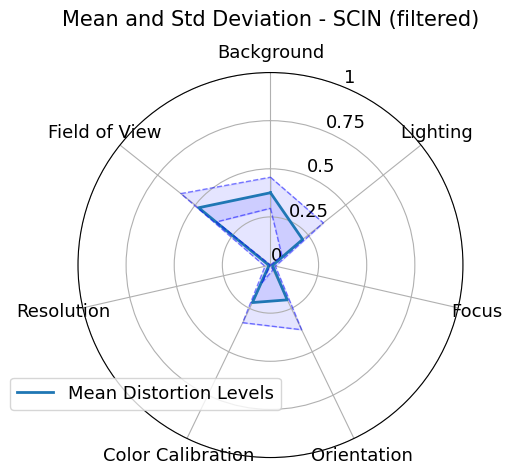
\includegraphics[width=\textwidth]{img/SCIN_hept.png}
        \caption{Filtered SCIN Images}
        \label{fig:scin_hept}
    \end{subfigure}
    \hfill
    \begin{subfigure}[b]{0.32\textwidth}
        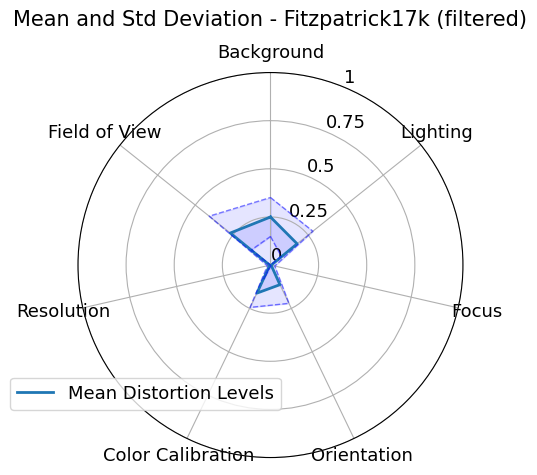
\includegraphics[width=\textwidth]{img/F17K_hept.png}
        \caption{Filtered Fitzpatrick Images}
        \label{fig:f17k_hept}
    \end{subfigure}
    \hfill
    \begin{subfigure}[b]{0.32\textwidth}
        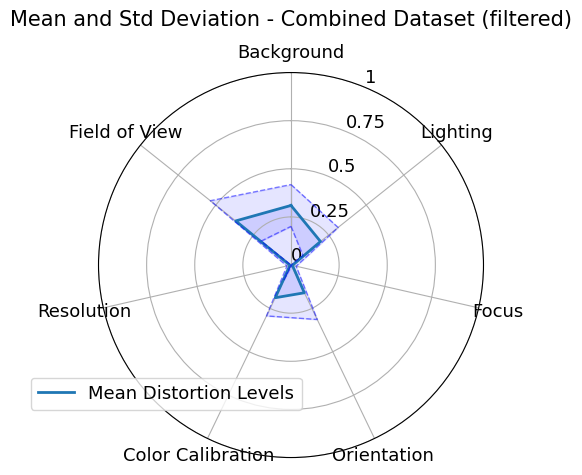
\includegraphics[width=\textwidth]{img/COMB_hept.png}
        \caption{Combined Images}
        \label{fig:comb_hept}
    \end{subfigure}
    \caption{Radar charts on the mean distortion levels and standard deviations across seven quality criteria for the 475 good quality SCIN, Fitzpatrick17k, and combined images.}
    \label{fig:hept}
\end{figure}